% \section{Experiments}\label{sec:experiments}

% \subsection{Experimental Setup}
% \shortparagraph{Dataset.} 
% To ensure a fair comparison across different rollout sampling strategies, we follow the Minimal-RL recipe~\citep{xiong2025minimalist} and train all models on the Numina-Math dataset~\citep{numina_math_7b}, which contains 860k math prompts paired with ground-truth answers. 
% %

% \shortparagraph{Models.}
% We conduct experiments with both Qwen-2.5-Math-1.5B~\citep{yang2024qwen2} and Llama-3.2-1B-Instruct~\citep{dubey2024llama}\footnote{We also experimented with the Llama-3.2-1B Base~\citep{dubey2024llama}; however, consistent with the observation of \citet{wang2025octothinker}, training base models with RL without proper mid-training (domain-specific fine-tuning) is challenging, yielding limited performance gains for all methods. We leave a more thorough investigation of this direction for future work.} to ensure generality, following the advice promoting rigorous RLVR evaluation~\citep{shao2025spurious, wu2025reasoning}. We additionally experiment with  Qwen-2.5-Math-7B model to see how well our methods generalize with model size scaling. 
% %

% \textbf{Baselines.}
% We evaluate \alg against standard fixed-temperature sampling with temperatures $\tau \in \{0.6, 1.0, 1.2\}$. 
% %
% % \zz{Should we mention these fixed-temp sampling are combined with GRPO, DAPO and GPG?}
% These values are chosen based on recommendations from prior work to establish strong baselines~\citep{renze-2024-effect, guo2025deepseek, hou2025t1}.
% %
% For a fair and controlled comparison, we disable two features for all methods: 
% (1) dynamic sampling~\citep{yu2025dapo}, to ensure all prompts are used during training;
% and (2) rollout length penalties, to avoid biasing the sampling process. 
% %
% As discussed in \cref{sec: method}, these techniques are orthogonal to our contribution and we leave further investigation about these to future work.
% %
% % \ych{Shall we demonstrate a case that with all techniques in place, using standard training recipe like DAPO, how well our model could be?}


% \shortparagraph{Implementation details.}
% Most experiments are conducted within DAPO~\citep{yu2025dapo} algorithms. To test whether \alg can apply to various RL algorithm, we additionally test \alg in GRPO~\citep{shao2024deepseekmath} and EntropyMech~\citep{cui2025entropy} using the same training and evaluation setup. 
% %
% More training details and hyperparameter setups are illustrated in \cref{app: minimal_rl_training_details}. 
% %
% Unless otherwise specified, we set $\tau_{\max}=1.2$ and $d=25$ as the default configuration for \alg.
% %
% We empirically find that for larger model with stronger generative capability, using an overly small $\tau_{\text{small}}$ would trigger the model to generate seemingly correct but wrong answers over the held-out validation set. 
% %
% For 1B models, we use $\tau_{\min}=0.1$ and we use $\tau_{\text{small}}=0.8$. All hyperparameters are tuned based on a prior study over held-out datasets. 
%
% \zz{might need to re-phrase since we only mention 1B models in this section, but I guess we are still waiting for llama 8B}


\section{Experiments}\label{sec:experiments}
\begin{figure}[t]
\centering
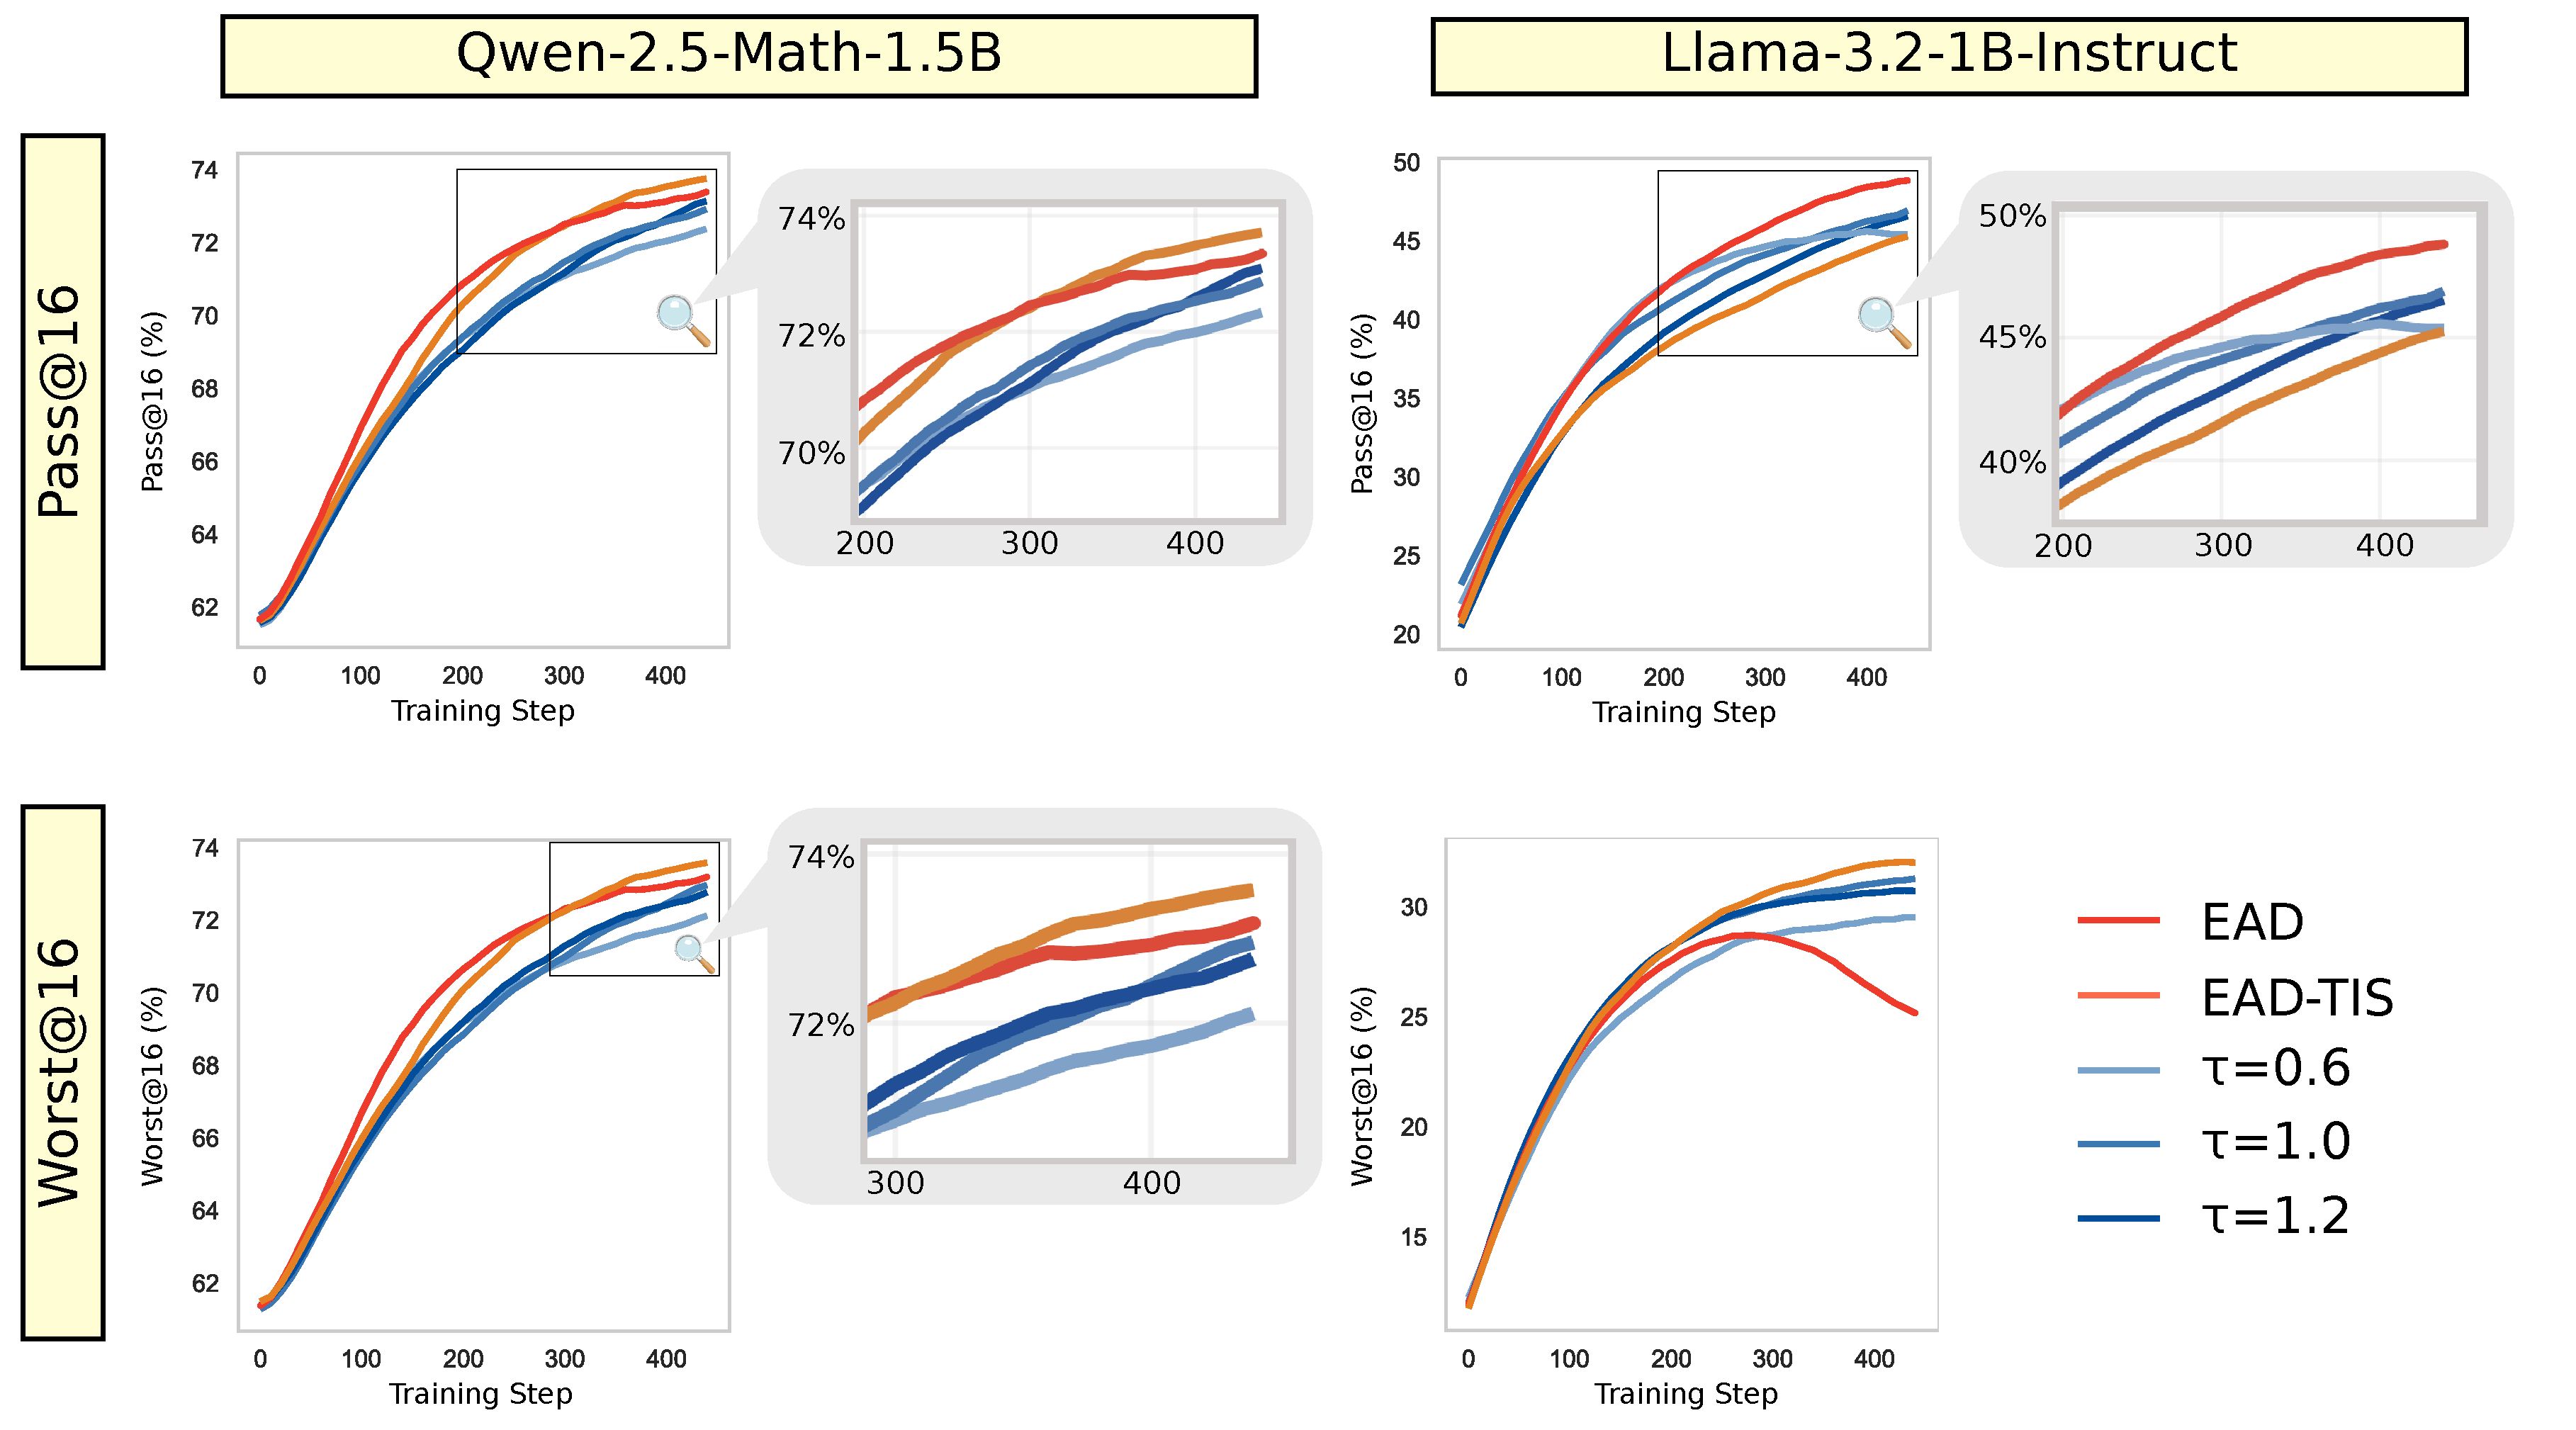
\includegraphics[width=\linewidth]{icml2026/figures/best-and-worst-at-16.pdf}
\caption{
Pass@16 and Worst@16 performance evaluation in RL training. 
While \alg improves exploration of high-quality samples (even the worst outperform temperature sampling), the gain diminishes over time; importance sampling can supplement to correct bias and sustain training.
}
\label{fig: main_bench_best_worst_at_16}
\vspace{-13pt}
\end{figure}
%
\begin{figure}[!ht]
    \centering
    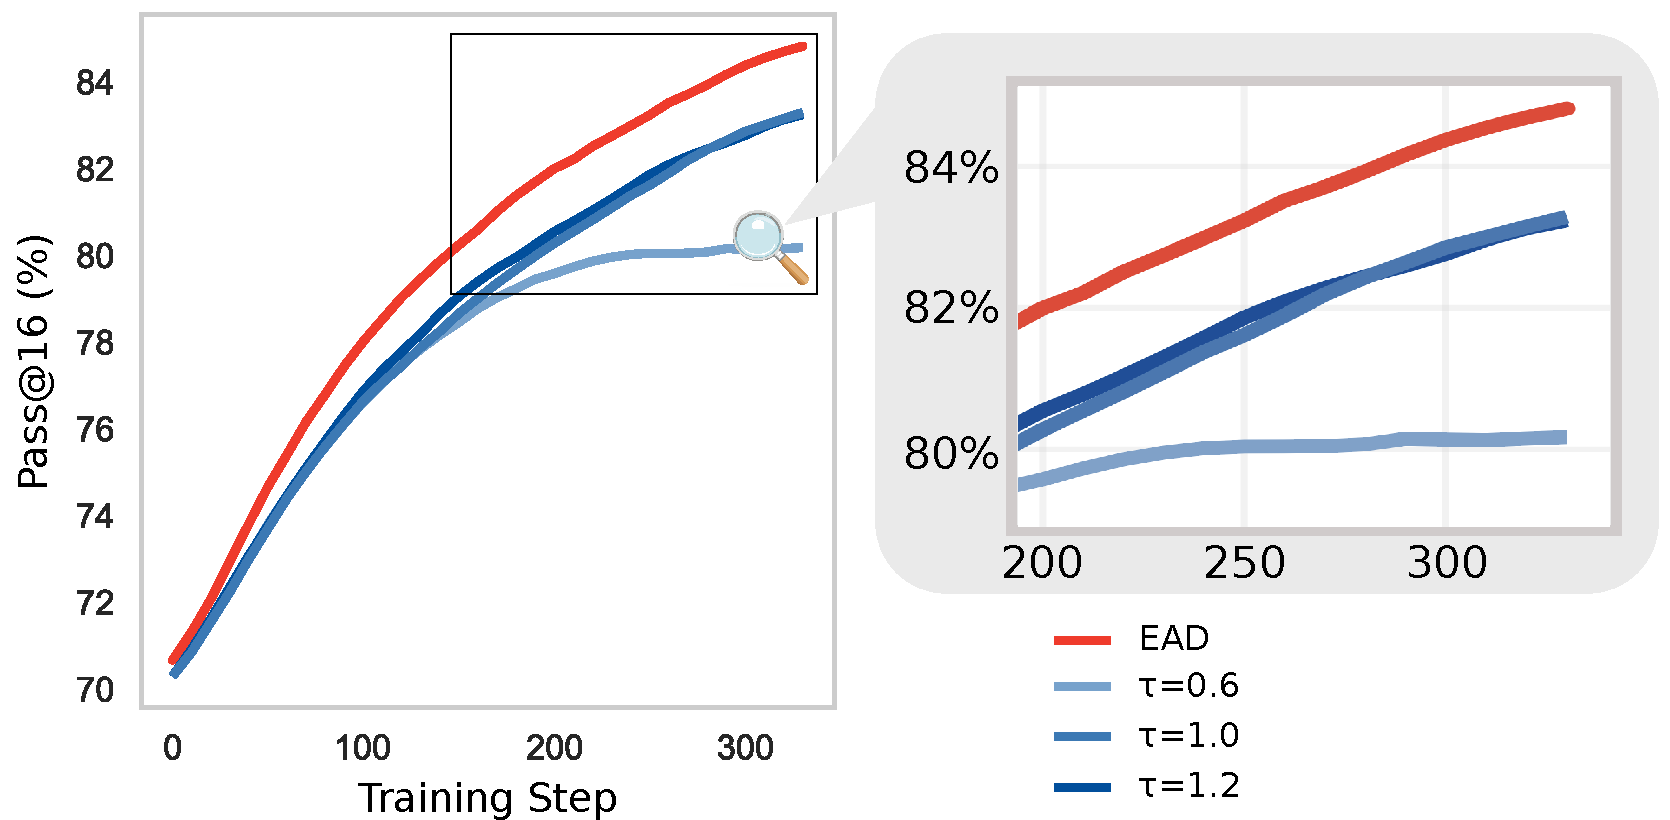
\includegraphics[width=0.6\linewidth]{icml2026/figures/best_at_16_Qwen2.5-Math-7B.pdf}
    \caption{
    % Qwen-2.5-7B
    Pass@16 performance on Qwen-2.5-Math-7B. 
    %
    \alg enables better exploration than fixed-temperature sampling, yielding sustained gains in Pass@16 throughout training.
    %
    }
    \label{fig: best_at_16_qwen2.5_7b}
    \vspace{-20pt}
\end{figure}
%

\subsection{Experimental Setup}
\label{sec: experiment_setup}
\shortparagraph{Models, Data, and Training Frameworks.}
To ensure a rigorous and controlled comparison, we follow the Minimal-RL recipe~\citep{xiong2025minimalist},\footnote{More training details and hyperparameter setups are illustrated in \cref{app: minimal_rl_training_details}. } training all models on the Numina-Math dataset~\citep{numina_math_7b}, which contains 860k math prompts. To assess the generality of our method, we experiment with both Qwen-2.5-Math-1.5B~\citep{yang2024qwen2} and Llama-3.2-1B-Instruct~\citep{dubey2024llama}.\footnote{We also experimented with the Llama-3.2-1B base model. However, consistent with \citet{wang2025octothinker}, we found that applying RL to base models without intermediate domain-specific fine-tuning yields limited gains across all methods. We defer a deeper investigation to future work.} We also include the larger Qwen-2.5-Math-7B model to evaluate how our approach scales. While our primary experiments are conducted within the DAPO framework~\citep{yu2025dapo}, we demonstrate broader applicability by additionally integrating \alg with GRPO~\citep{shao2024deepseekmath} and EntropyMech~\citep{cui2025entropy}.

\shortparagraph{Baselines and Controlled Comparison.}
We evaluate \alg against fixed-temperature sampling, with temperatures $\tau \in \{0.6, 1.0, 1.2\}$ as recommended by prior work~\citep{renze-2024-effect, guo2025deepseek, hou2025t1}. For a fair comparison focused specifically on the sampling strategy, we disable two orthogonal techniques for all methods: (1) dynamic data sampling~\citep{yu2025dapo}, to maintain a consistent training set, and (2) rollout length penalties, to avoid confounding the reward signal with length-based biases.

\shortparagraph{Hyperparameters.}
Unless otherwise stated, we use a default configuration of $\tau_{\max}=1.2$, $d_0=25$, $\alpha = 5$, and $d_{\max}=40000$ for \alg. 
%
For $\tau_{\min}$, we observed optimal values varied by model capability.
%
For the 1B and 1.5B models, we set $\tau_{\min}=0.1$. 
%
For the more capable 7B model, we used a higher value of $\tau_{\min}=0.8$.
%
All hyperparameters are tuned based on a prior study over held-out datasets. 
%

% \subsection{\algname Improves RLVR Performance}
\subsection{\alg Improves RLVR Training}

\shortparagraph{\alg Improves RL Exploration and Training Efficiency.}
As shown in \cref{fig: main_bench_best_worst_at_16}, \alg significantly improves training efficiency. 
%
For Pass@16 accuracy, 
% both \alg (w/o TIS) and \alg (w/ TIS) 
\alg (w/o TIS) consistently outperforms the baselines on the Llama and Qwen models (\alg (w/ TIS) also outperforms on the Llama model), demonstrating more effective exploration. 
%
Under the stricter Worst@16 metric, the inclusion of TIS becomes essential for maintaining stable performance gains, highlighting its importance for correcting the off-policy training dynamic introduced by \alg. 
%
Through bootstrapping evaluation as in~\citet{hochlehnert2025sober}, the standard deviation of both Pass@16 performance and Worst@16 are way below 0.01 and thus all comparisons here are significant.
%

To verify that our method generalizes, we evaluated it on the larger Qwen-2.5-Math-7B model. The results, presented in \cref{fig: best_at_16_qwen2.5_7b}, confirm that the performance gains from \alg remain significant. This demonstrates that our approach is effective not only on smaller models but also scales successfully.
%


\shortparagraph{\alg Mitigates Entropy Collapse.}
One major problem in RLVR training is entropy collapse~\citep{cui2025entropy}, which shrinks the exploration space and constrains improvement during the ``plateau stage''~\citep{deng2025trial}.
%
We plot the entropy dynamic in \cref{fig: main_bench_entropy}, where we can see that the entropy dynamic for \alg-empowered methods is not monotonically decreasing from the beginning. 
%
Instead, it tries to gradually transition out from local optimum~\citep{kirkpatrick1983optimization, bertsimas1993simulated} in a natural, continuous way without any external intervention, such as introducing tree search in rollout sampling~\citep{li2025treepo}.
%

\shortparagraph{Sample efficiency of \alg.}
Increasing the number of rollouts is a common but computationally expensive strategy to enhance exploration~\citep{hou2025t1}. 
%
We test the sample efficiency of \alg by varying the number of rollouts, adjusting the learning rate accordingly as suggested by prior work~\citep{chen2025pass}. 
%
As shown in \cref{fig: main_bench_rollout_scaling}, while more rollouts can further improve performance, \alg achieves strong results with just 4 or 8 rollouts. 
%
For instance, the optimal configurations are $n=8$ with a learning rate of $10^{-6}$ for Llama-3.2-1B-Instruct and $2\times10^{-6}$ for Qwen-2.5-Math-1.5B. 
%
This highlights the sample efficiency of our approach, offering a way to reduce the computational cost of the rollout phase.
%



To assess whether \alg's advantage persists with extensive exploration, we compare it against baselines using a larger set of 16 rollouts. 
%
\cref{fig: rollout_modelwise_compare} shows that although the relative performance gain diminishes, \alg still outperforms fixed-temperature baselines by a clear margin.
%
\subsection{\alg is Compatible with Various RL Algorithms}
To demonstrate that \alg is a general, plug-and-play exploration strategy, we evaluate its performance when integrated into two other prominent RL algorithms: GRPO~\citep{shao2024deepseekmath} and EntropyMech~\citep{cui2025entropy}. 
%
These algorithms provide diverse testbeds. 
%
GRPO is more conservative, constraining policy updates with a KL divergence penalty and stricter clipping mechanism that can limit exploration~\citep{yu2025dapo}, while EntropyMech uses a specialized token-clipping mechanism to mitigate entropy collapse. 

%
As shown in \cref{fig: algorithm_wide_comparison}, \alg consistently outperforms fixed-temperature sampling in both frameworks. 
%
These results confirm the broad applicability of our method as an improved exploration strategy across different RL algorithms.

\begin{figure}[t]
    \centering
    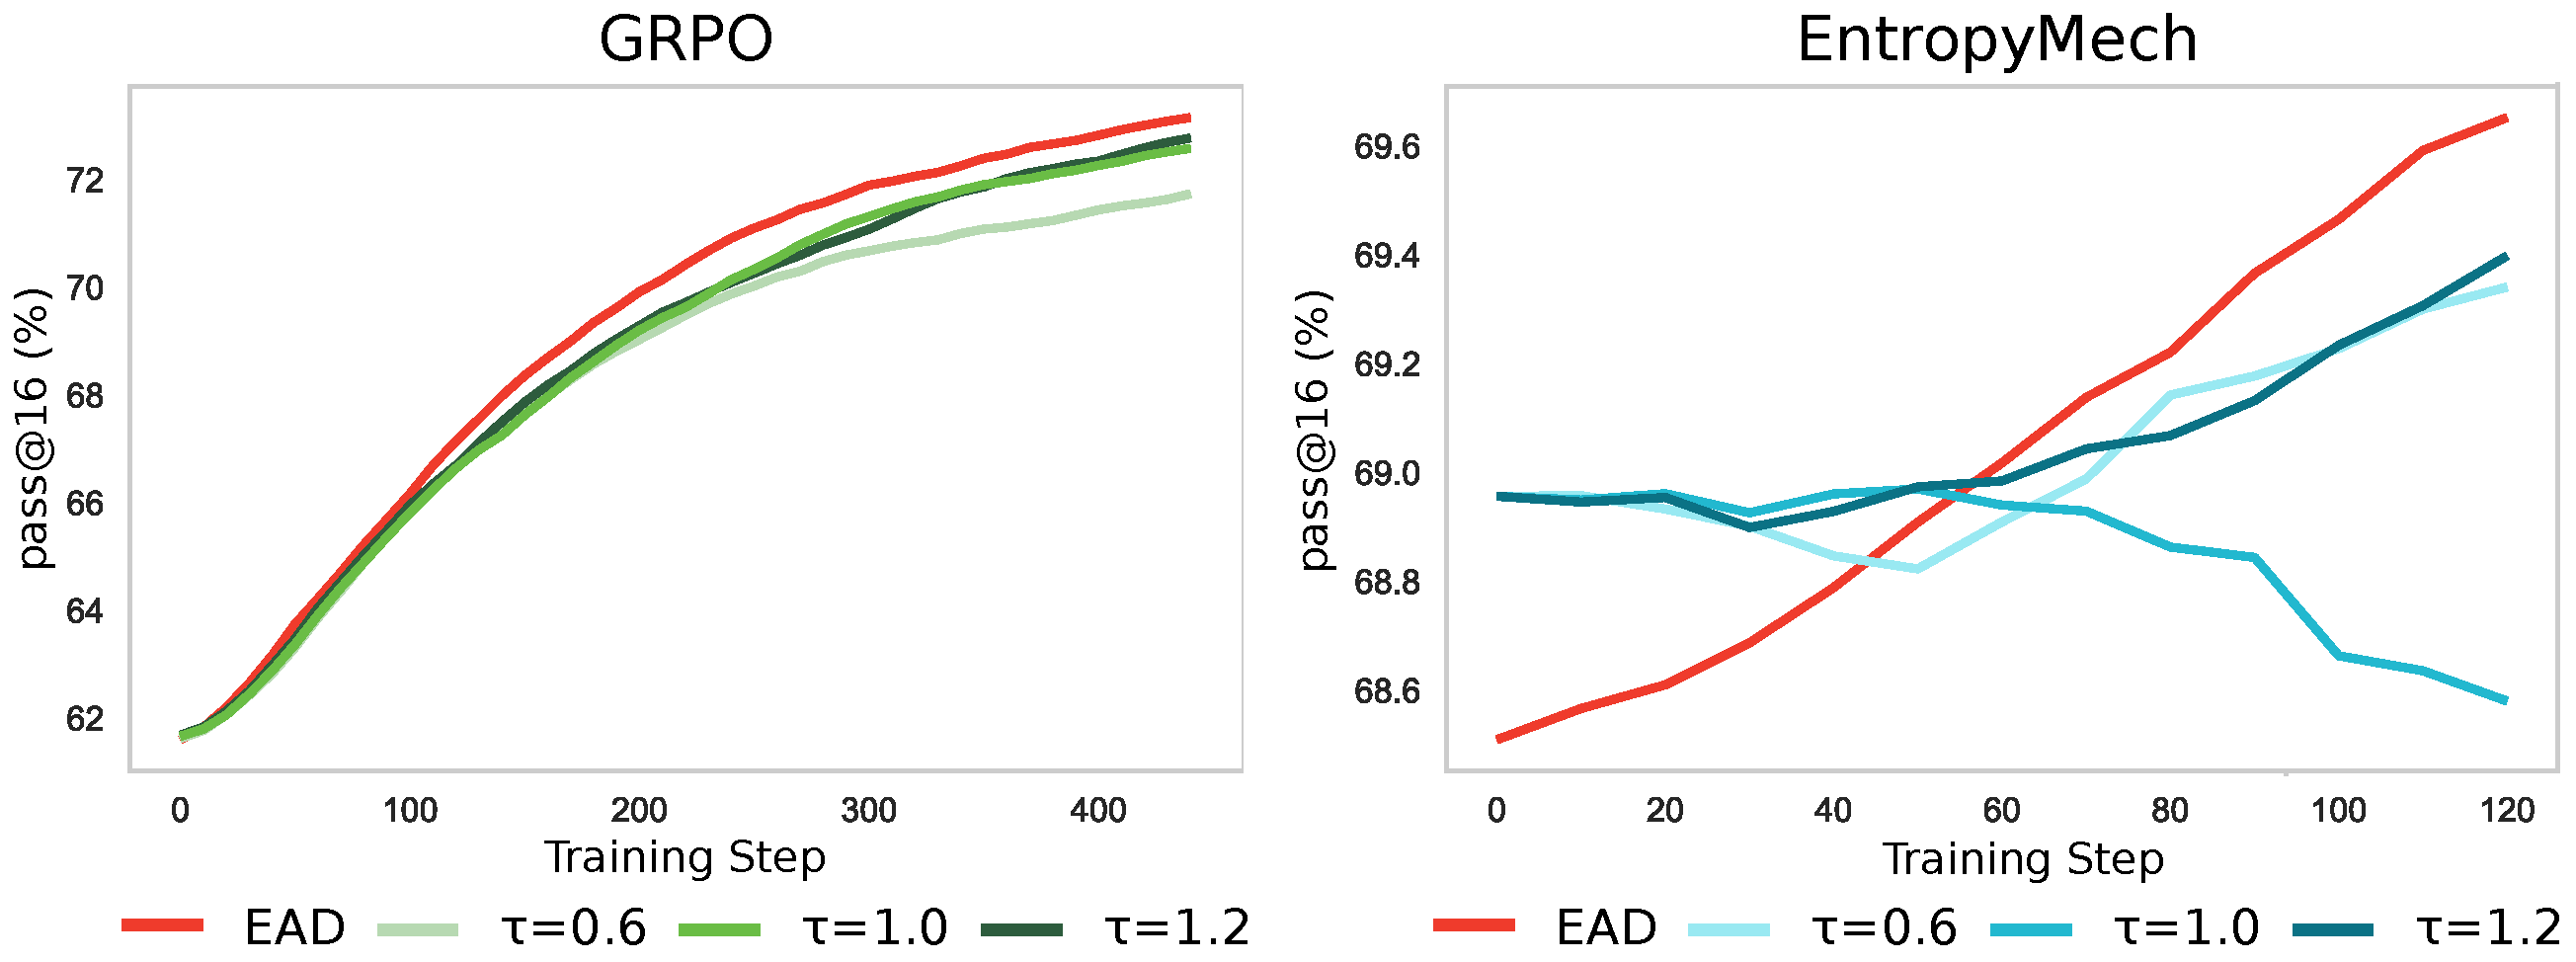
\includegraphics[width=\linewidth]{icml2026/figures/diff-method.pdf}
    \caption{\alg is compatible with various RL algorithms and can significantly improve the model performance over time. } 
    \label{fig: algorithm_wide_comparison}
    \vspace{-10pt}
\end{figure}
%
\begin{figure}[!ht]
    \centering
    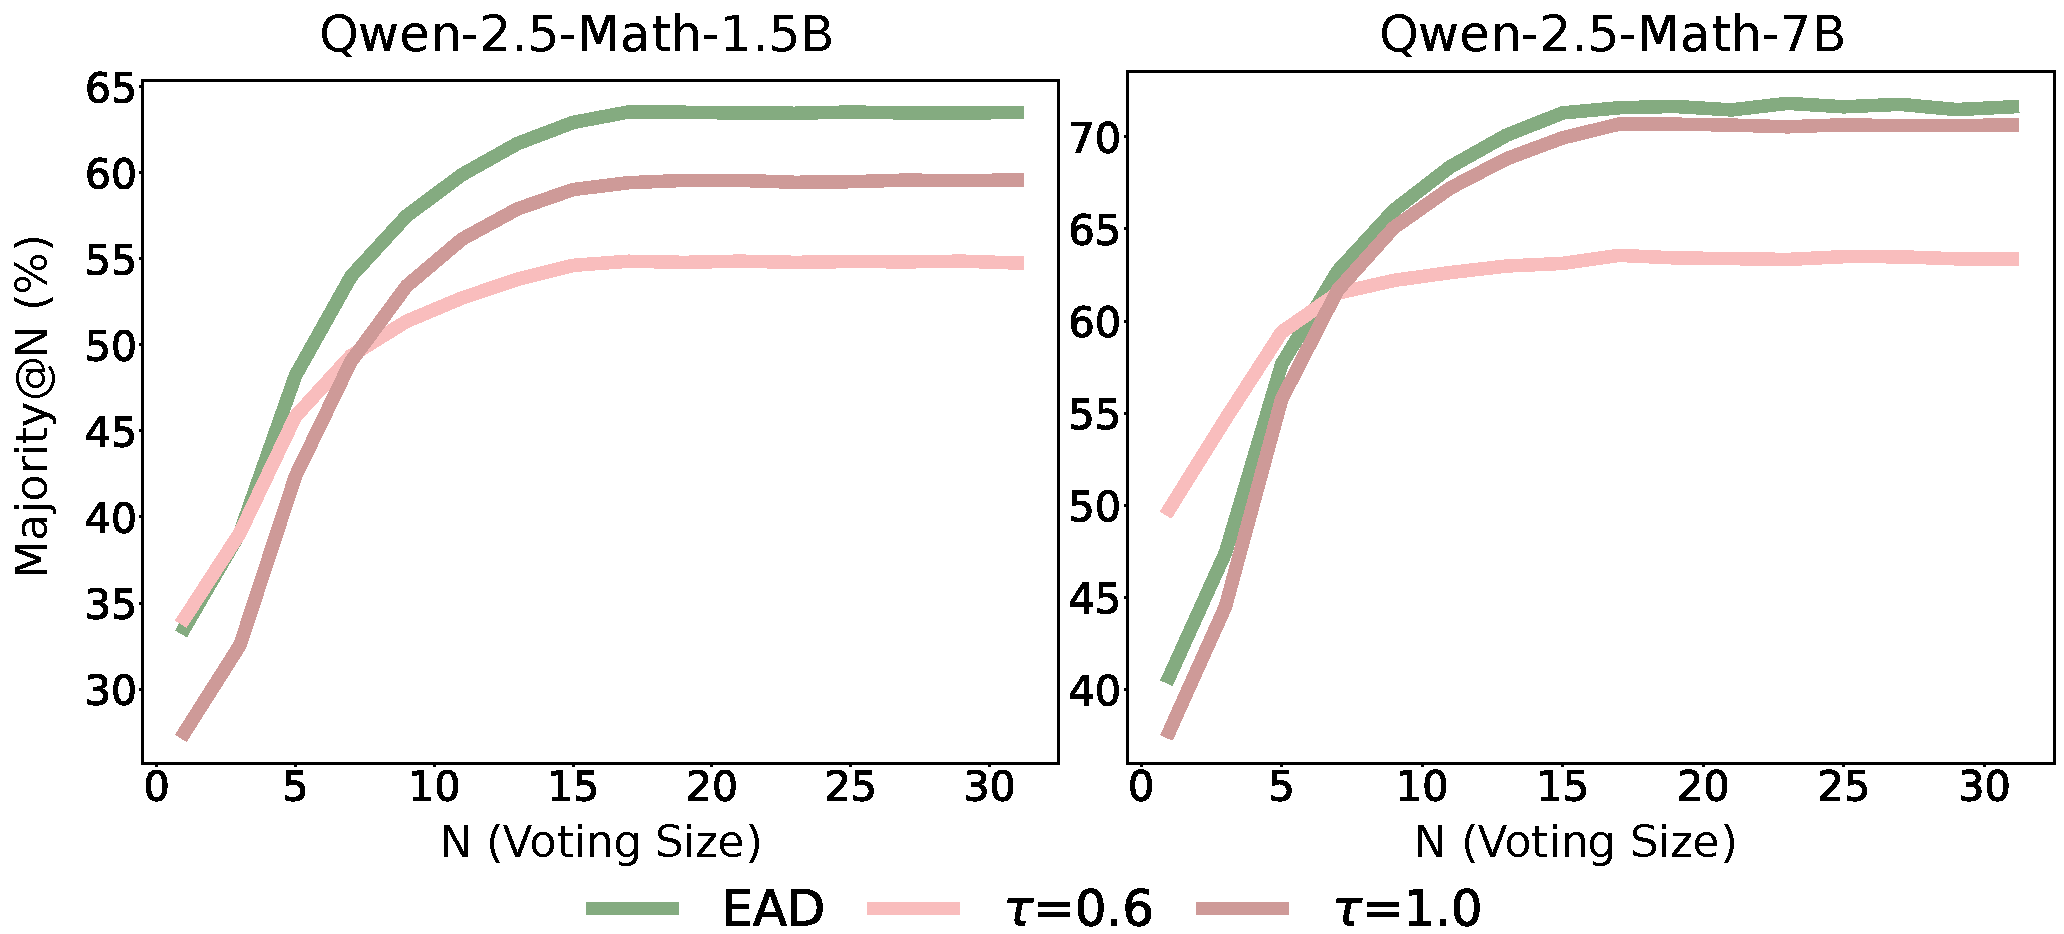
\includegraphics[width=\linewidth]{icml2026/figures/inference-time-scaling.pdf}
    \caption{Inference-Time Scaling Evaluation for Different Decoding Methods using off-the-shelf Qwen2.5 models. We could see that \alg improves traditional temperature sampling. We set $\tau_{\text{max}}=1.2, \tau_{\text{min}}=0.1, d=25$ for \alg. }
    \label{fig: inference_time_scaling}
    \vspace{-15pt}
\end{figure}
%
\begin{figure}[t]
    \centering
    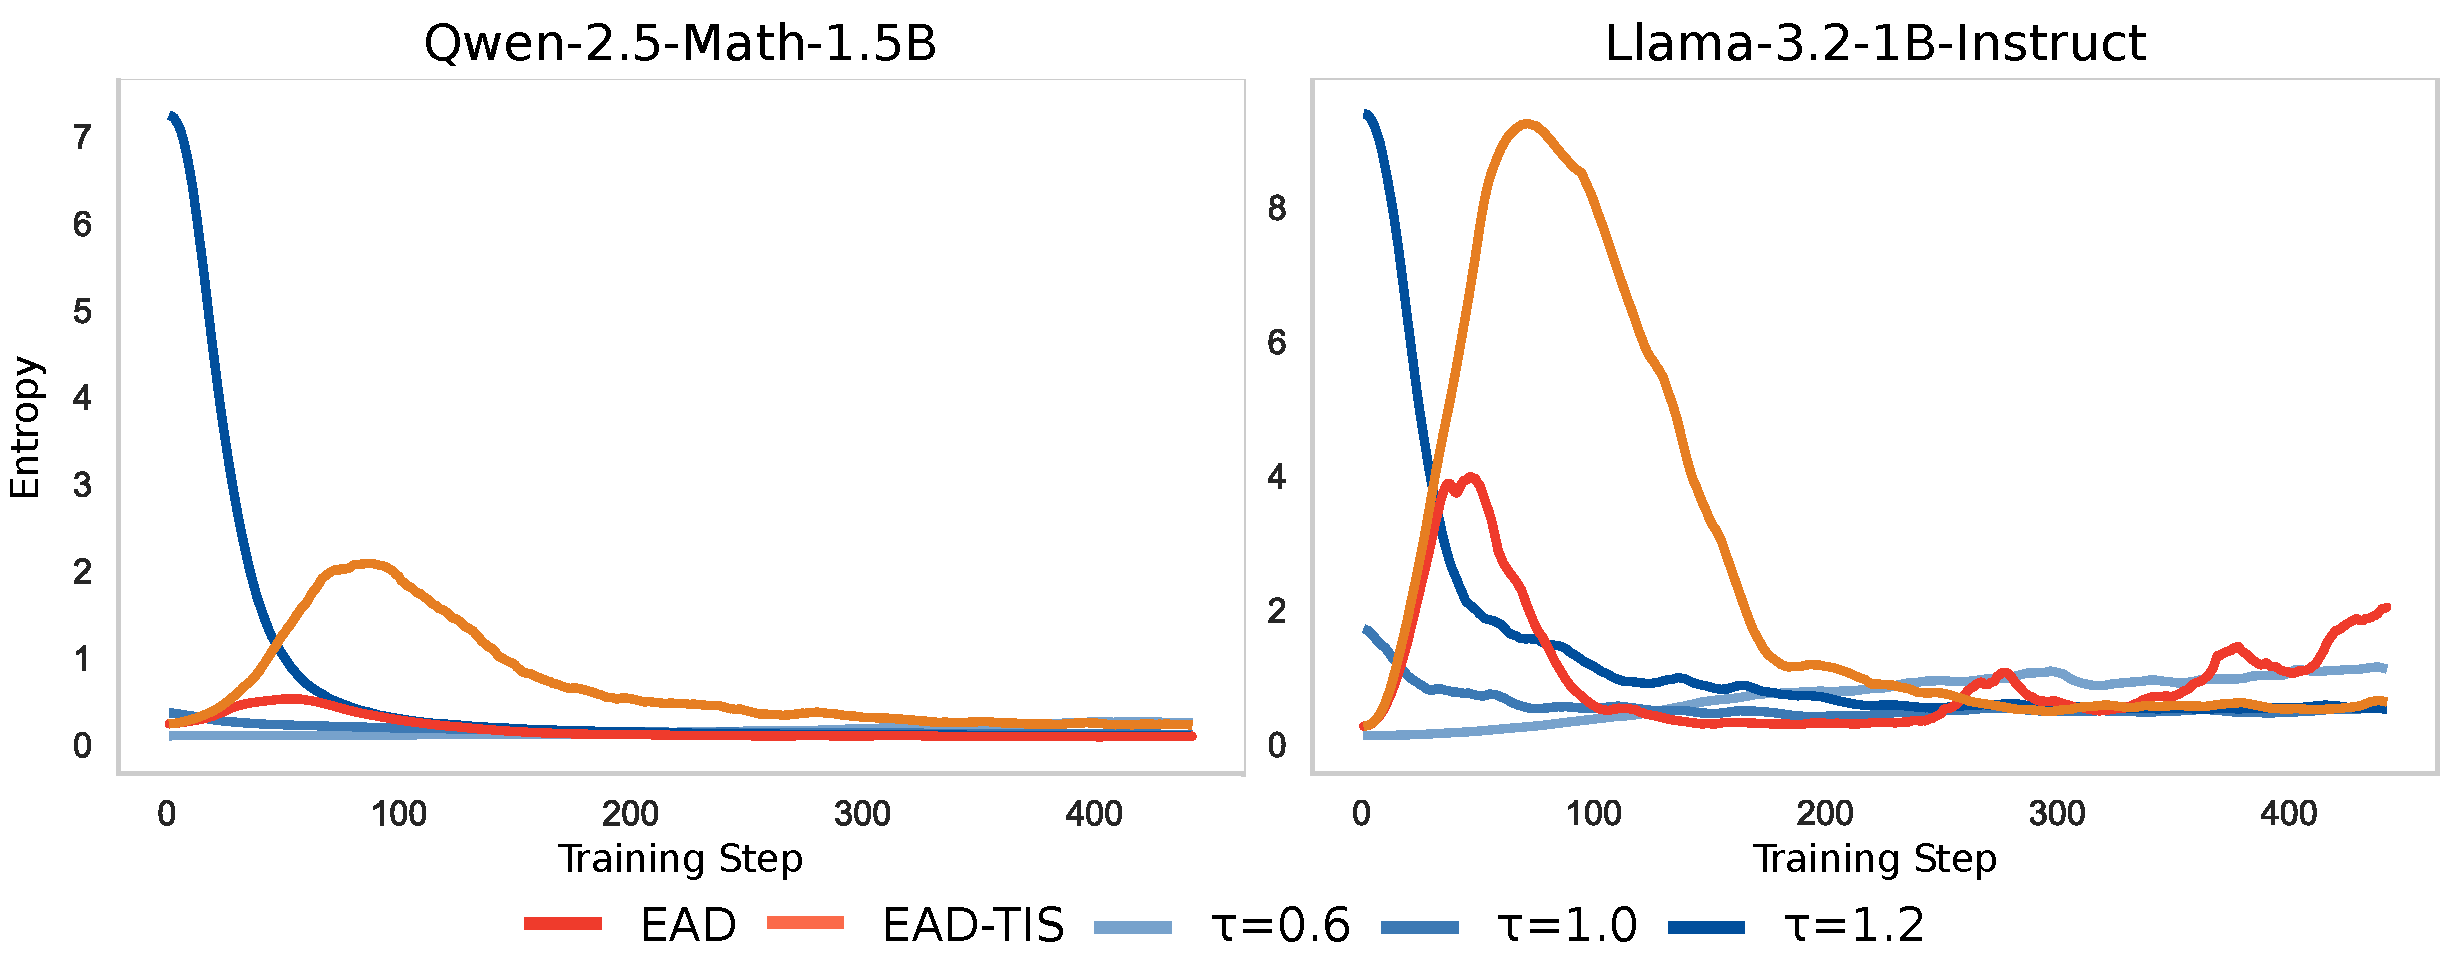
\includegraphics[width=\linewidth]{icml2026/figures/entropy.pdf}
    \caption{Entropy dynamics in RL training. With fixed temperature sampling, entropy decreases sharply from the start, limiting exploration. EAD helps the algorithm escape local minima by enabling exploration when needed during training.}
\label{fig: main_bench_entropy}    \vspace{-5pt}
\end{figure}

\begin{figure}[h!]
\begin{subfigure}{\linewidth}
    \centering
    % \vspace{-0.1in}
    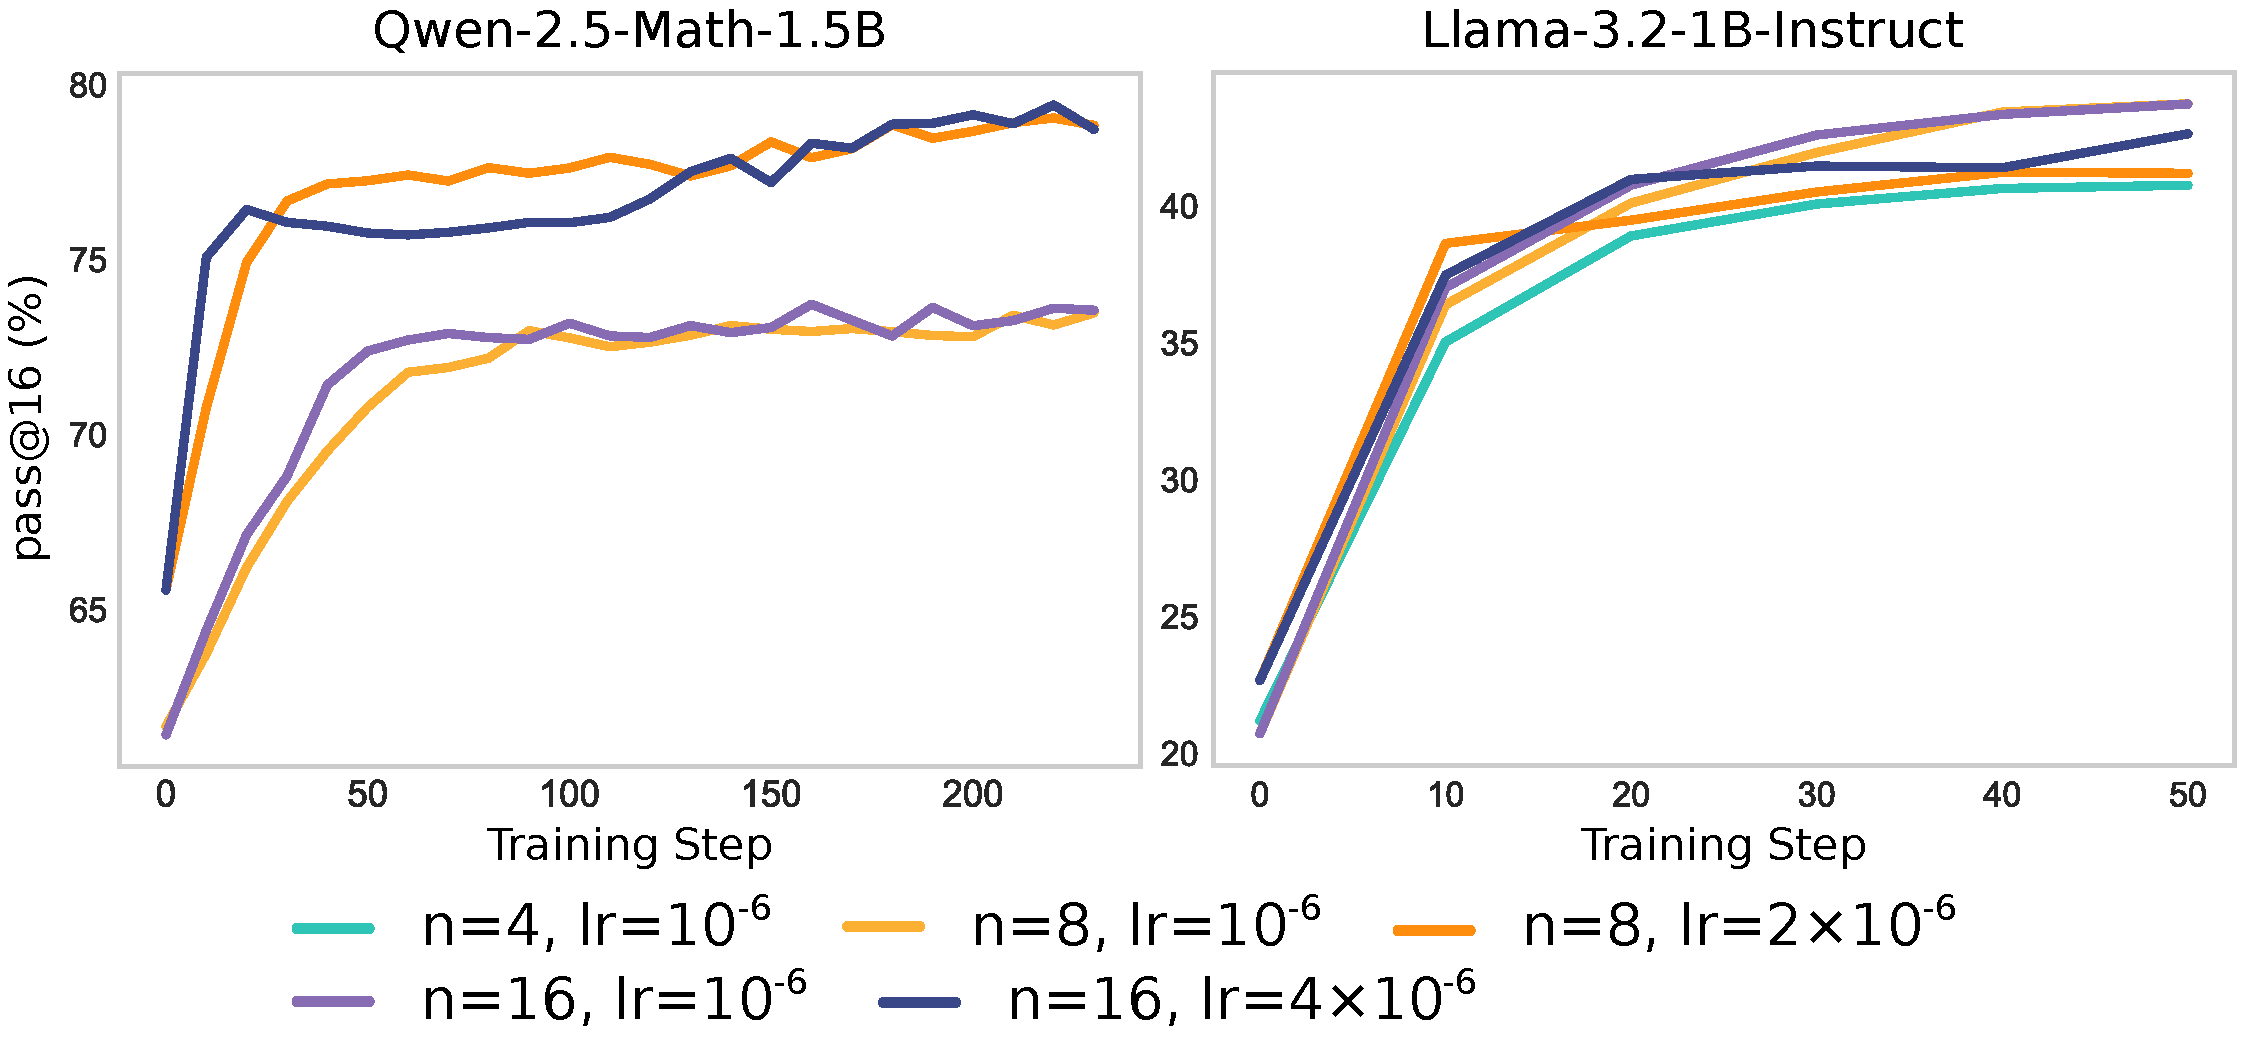
\includegraphics[width=\linewidth]{icml2026/figures/scaling-rollout.pdf}
    % \vspace{-0.15in}
    \caption{\alg would bring further performance improvement via increased numbers of rollouts, but the commonly used $4$ or $8$ is already good enough. }
    \label{fig: main_bench_rollout_scaling}
% \vspace{-0.4in}
\end{subfigure}
% \end{figure}
\begin{subfigure}{\linewidth}
% \begin{figure}[h!]
    % \vspace{-0.4in}
    \centering
    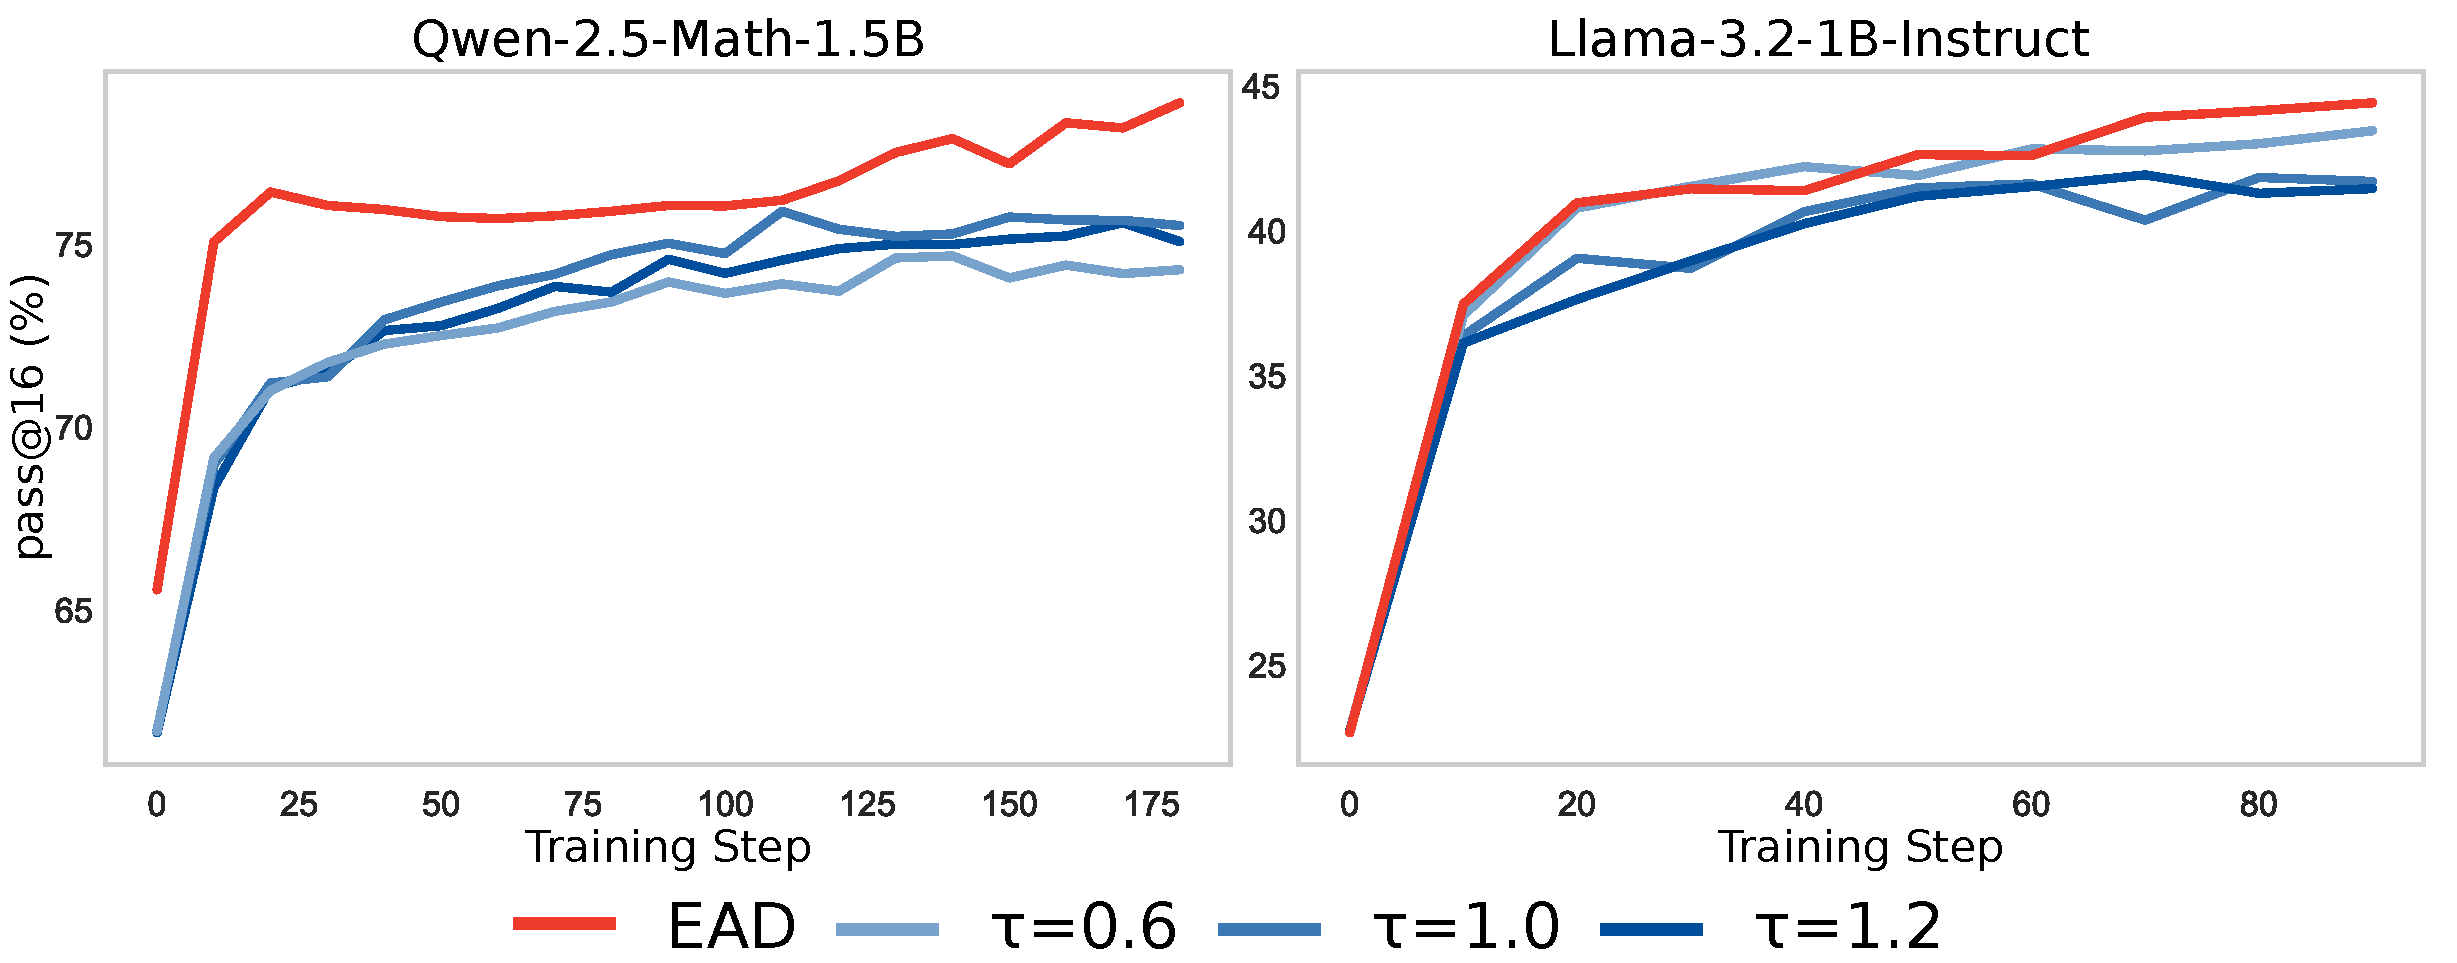
\includegraphics[width=\linewidth]{icml2026/figures/rollout-16-modelwise-compare.pdf}
    % \vspace{-0.25in}
    \caption{When scaling out the rollout number to 16, the relative advantages of our methods diminished; however, it still outperforms traditional same-temperature sampling.}
    \label{fig: rollout_modelwise_compare}
    % \vspace{-0.1in}
% \end{figure}
\end{subfigure}
\caption{Sample Efficiency of EAD. }
\vspace{-0.10in}
\end{figure}

\subsection{\alg Improves Inference-Time Scaling}
%
To understand whether the success of \alg in RL training is driven by its ability to generate high-quality samples, we conduct an evaluation at inference time. 
%
This experiment is designed to isolate the sampling strategy's effectiveness from the dynamics of RL optimization~\citep{berseth2025exploration}. 
%
Using off-the-shelf Qwen-2.5 models without any fine-tuning, we compare \alg against fixed-temperature sampling. 
%
We use majority voting ($\text{Majority}@N$) to measure how performance scales with the number of samples $N$~\citep{wang2023selfconsistency, snell2024scaling}. 
%
As shown in \cref{fig: inference_time_scaling}, \alg consistently improves over the baseline for most values of $N$. 
%
This result confirms that \alg's advantage stems from its inherent capacity to discover higher-quality solutions, even without any training.
%

\subsection{Ablation Study}

\begin{figure}[t]
    \centering
    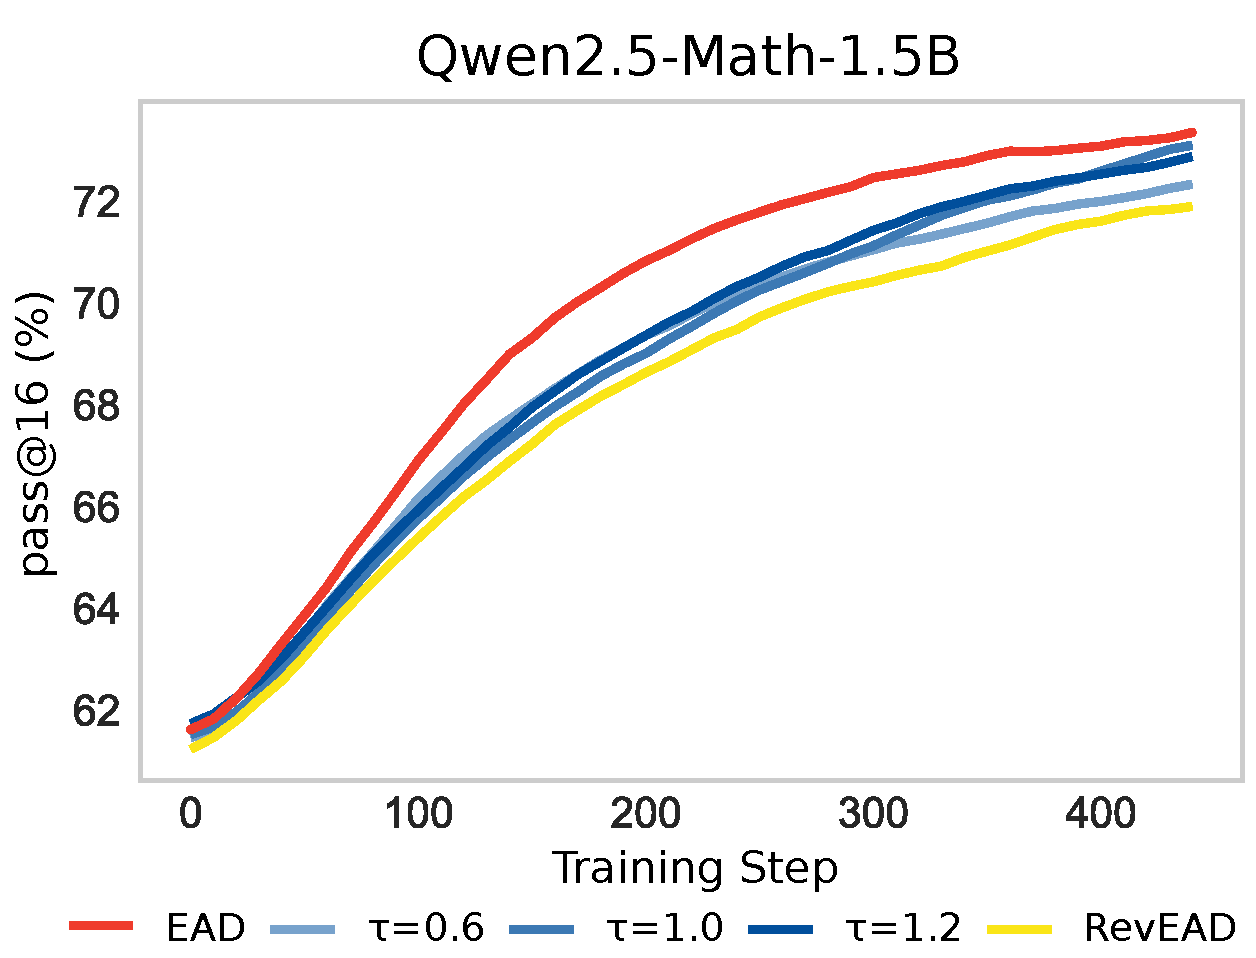
\includegraphics[width=0.66\linewidth]{icml2026/figures/reverse-annealing.pdf}
    \caption{Reverse Annealing experiment results. The reverse schedule fails to surpass normal temperature sampling.} 
    \label{fig: reverse_annealing}
    \vspace{-13pt}
\end{figure}

\begin{figure}[h!]
     \centering
     \begin{subfigure}[h]{0.235\textwidth}
         \centering
\vspace{-14pt}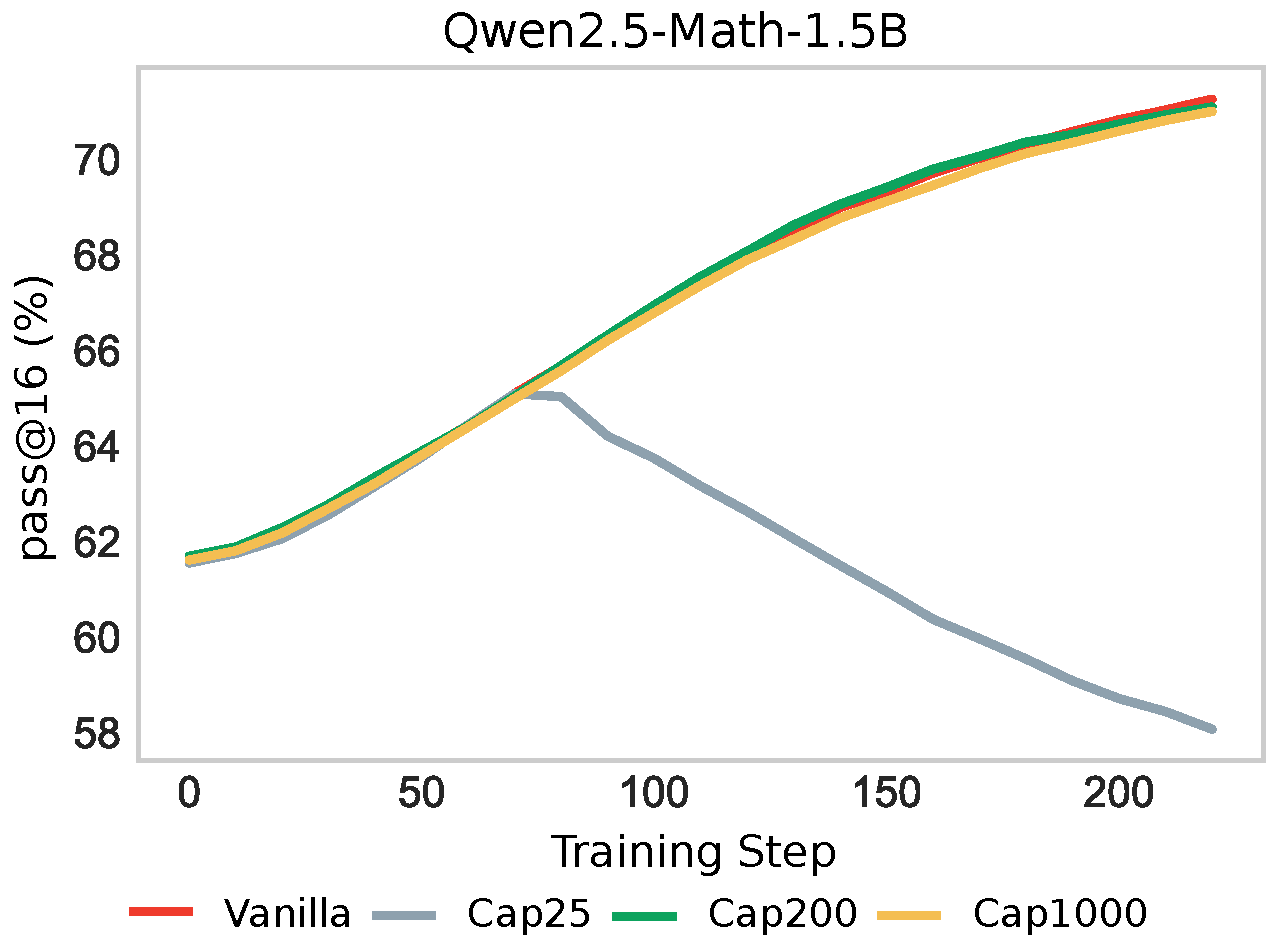
\includegraphics[width=\textwidth]{icml2026/figures/ablation-cap.pdf}
         \caption{Decay cap $d_{\max}$.}
         \label{fig: ablation_cap}
     \end{subfigure}
     \begin{subfigure}[h]{0.235\textwidth}
         \centering
         % \vspace{-0.1in}
         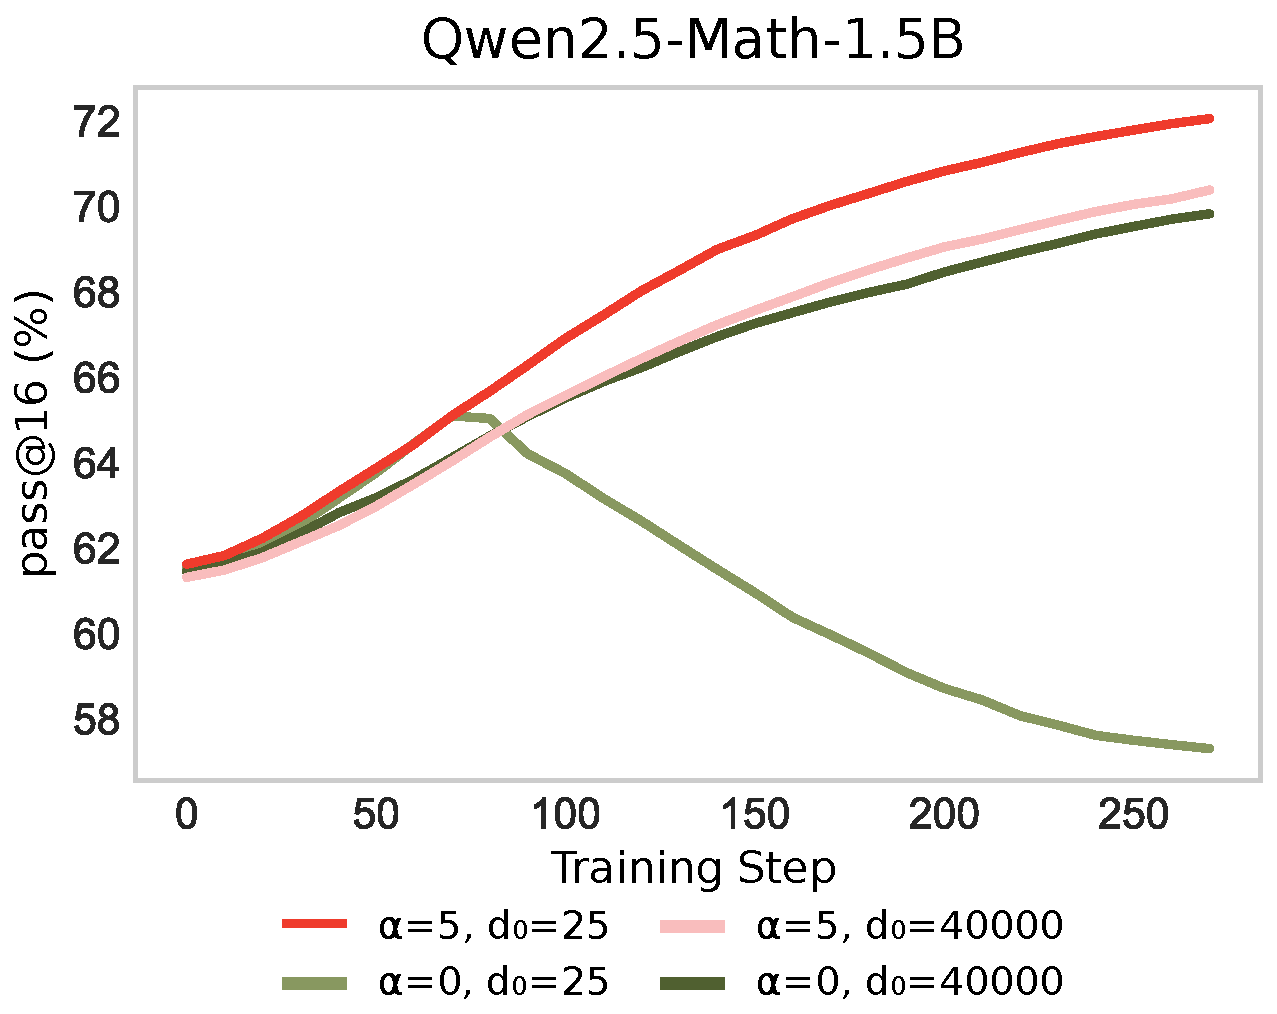
\includegraphics[width=\textwidth]{icml2026/figures/ablation-growth-factor-and-decay-freq-init.pdf}
         % \vspace{-3pt}
         \caption{Growth factor $\alpha$ and initial decay $d_0$.}
         \label{fig: ablation_growth_factor_and_decay_freq_init}
     \end{subfigure}
\caption{Ablation on hyperparameter sensitivity. \textbf{Left:} Ablation on decay cap $d_{\max}$. ``Vanilla'' denotes EAD with the default $d_{\max}=40000$. Setting $d_{\max}=25$ (where $d_0=25$) mimics a fixed temperature schedule (effectively $\alpha=0$), leading to performance drops as the schedule fails to adapt to longer responses. \alg remains robust provided $d_{\max}$ allows for smooth temperature reduction (e.g., $d_{\max} \ge 200$). \textbf{Right:} Ablation on growth factor $\alpha$ and initial decay $d_0$. With a small $d_0$, a positive growth factor ($\alpha > 0$) is required to adapt to increasing response lengths and maintain a smooth intra-sequence schedule. While a large $d_0$ ensures smoothness even with $\alpha=0$, it limits exploration, resulting in lower learning efficiency.}
\label{fig:hyper-parameter-sensitivity}
\vspace{-20pt}
\end{figure}

\shortparagraph{Reverse Annealing} We also test a reverse schedule, dubbed ``RevEAD'', where temperature increases during generation:
$\tau_t = \min\{\tau_\mathrm{min} + e^{t/d}, \tau_\mathrm{max}\}$.
As shown in \cref{fig: reverse_annealing}, RevEAD fails to even outperform standard temperature sampling, validating the necessity of an annealing (decreasing) temperature schedule. \revise{This observation also supports our hypothesis that late-stage exploration can be detrimental, potentially leading to high-variance ``lucky'' successes rather than robust reasoning paths.}

\shortparagraph{Hyperparameter Sensitivity} 
We conduct an ablation study on the decay cap $d_{\max}$ and the growth factor $\alpha$. As shown in \cref{fig: ablation_cap}, \alg is robust to a wide range of $d_{\max}$ values, provided the cap is sufficiently large to ensure a smooth annealing schedule. Conversely, a very small cap (e.g., $d_0=d_{\max}=25$) approximates a fixed schedule (equivalent to $\alpha=0$ throughout training). This setting causes an abrupt performance drop, likely because the model cannot adapt to the increasing response lengths during training (see \cref{app: increased_length}). Alternatively, using a large initial $d_0$ yields a smooth schedule even with $\alpha=0$. However, while training remains stable, performance improves slowly due to overly conservative exploration, as shown in \cref{fig: ablation_growth_factor_and_decay_freq_init}.


\subsection{Stress Test: DAPO-17K Recipe for AIME24}
To verify the effectiveness of \alg on realistic mathematical reasoning tasks, we stress-test it using the DAPO recipe~\citep{yu2025dapo}, training on DAPO-17k and evaluating on the challenging AIME 2024 benchmark. To accommodate GPU memory constraints, we utilize the Qwen-3-8B-Base~\citep{yang2025qwen3} model (instead of 32B) and reduce the maximum response length from 20480 to 8192. We set $d_0=500$ and $d_{\max}=40000$, and vary $\alpha \in \{5, 50\}$. As shown in \cref{fig: aime24}, \alg achieves significant learning efficiency and consistently outperforms the standard temperature sampling baseline.


\begin{figure}[t]
    \centering
    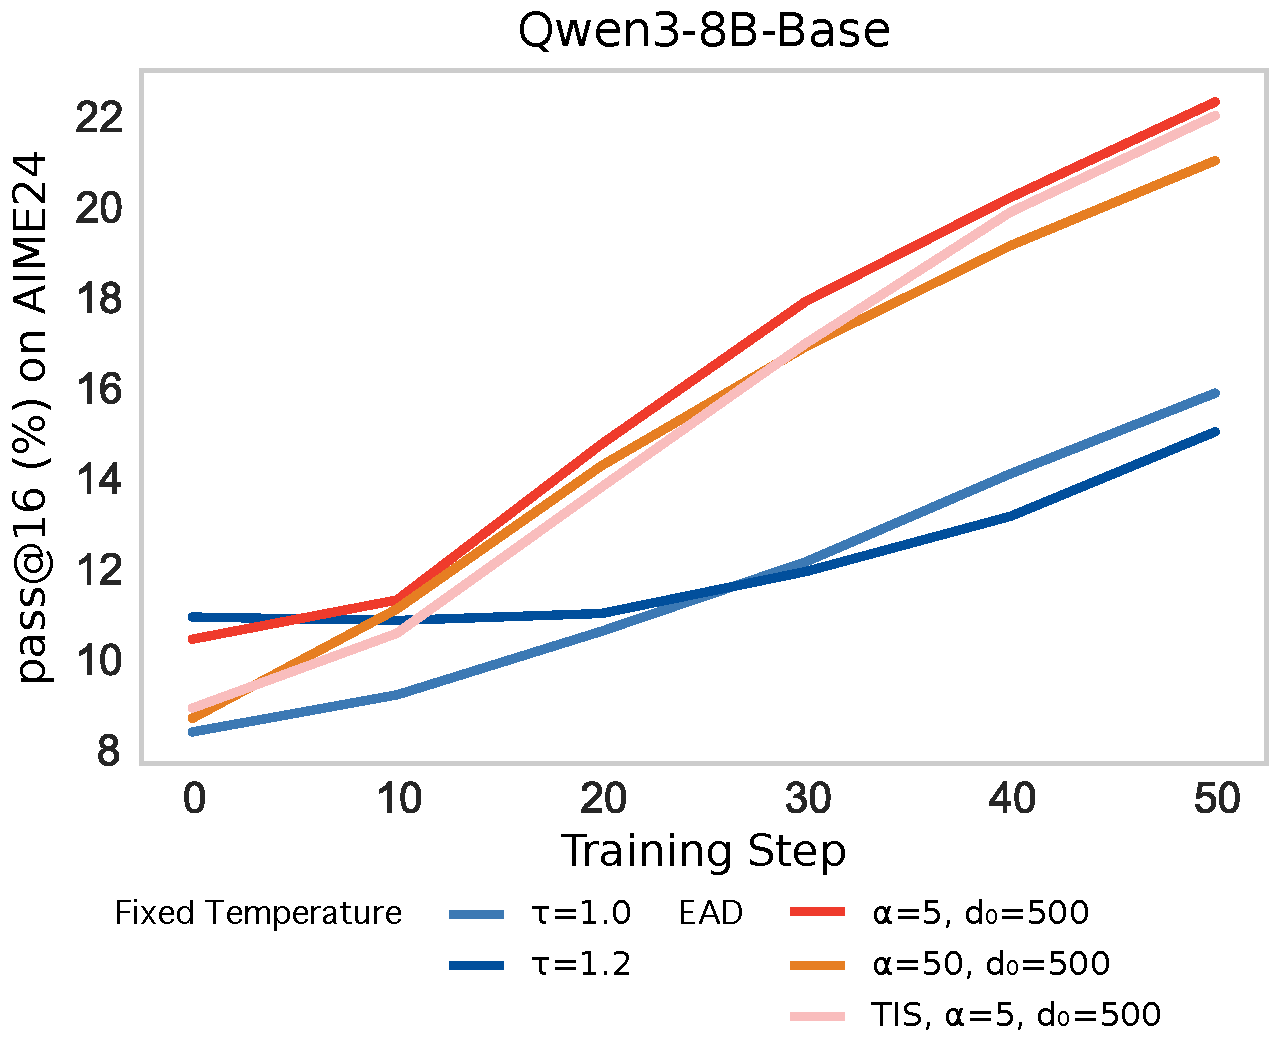
\includegraphics[width=0.66\linewidth]{icml2026/figures/aime24.pdf}
    \caption{Stress-test of \alg using the DAPO recipe on AIME24. \alg outperforms the temperature sampling baseline across various hyperparameter setups.} 
    \label{fig: aime24}
    \vspace{-20pt}
\end{figure}

% \begin{wrapfigure}{r}{0.39\textwidth}
% \vspace{-0.75in}
% % \begin{figure}[t]
%     \centering
%     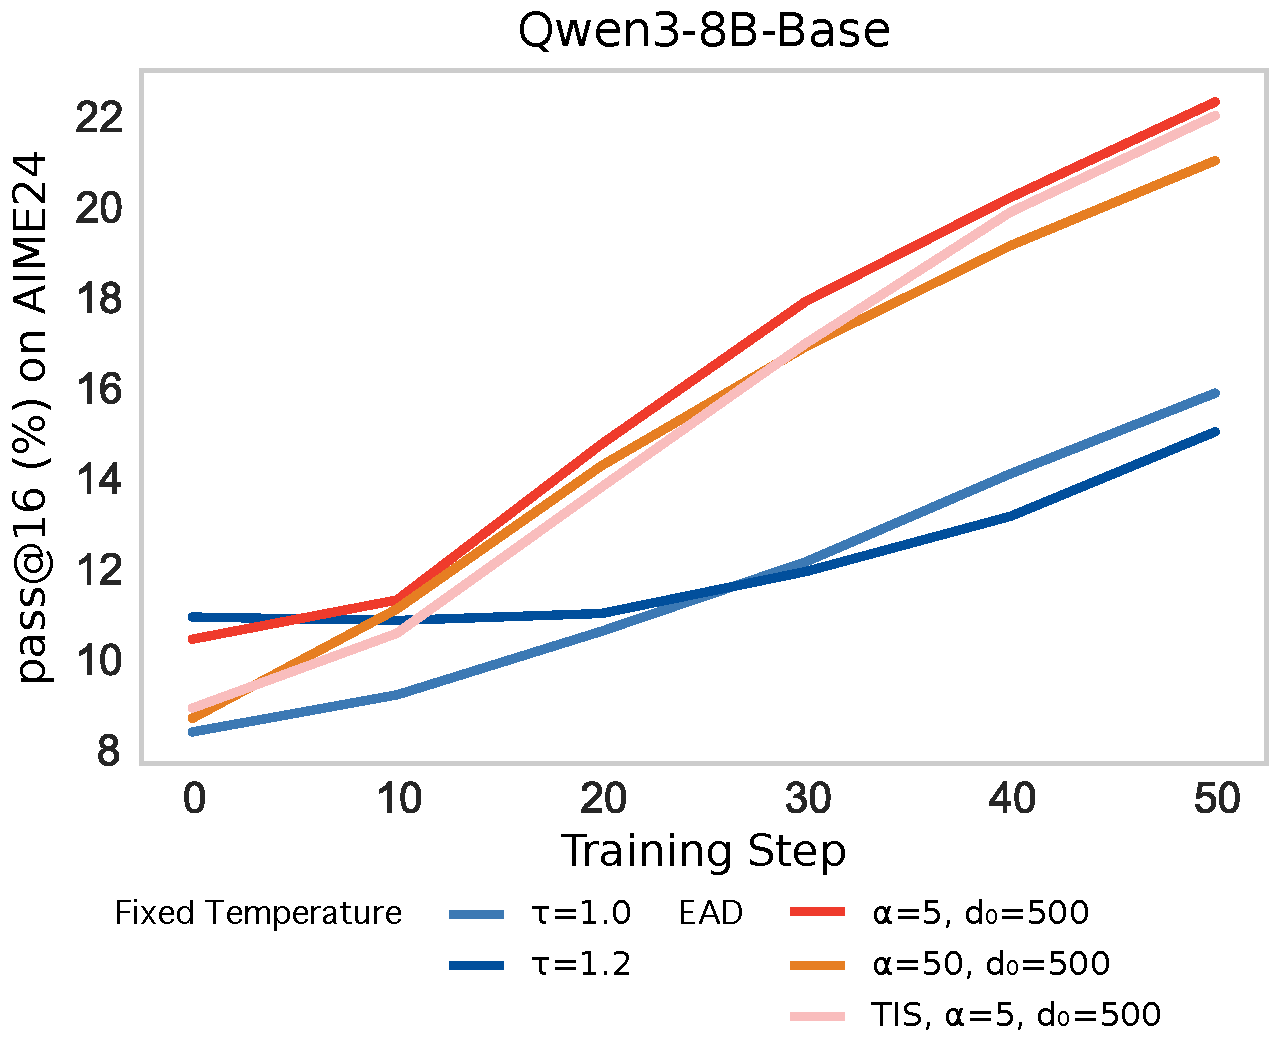
\includegraphics[width=\linewidth]{iclr2026/figures/stress_test_dapo16k/best_at_16_Qwen3-8B-Base-new.pdf}
%     % \vspace{-0.2in}
%     \caption{Stress-test of \alg using the DAPO recipe on AIME24. \alg outperforms the temperature sampling baseline across various hyperparameter setups.
%     } 
%     \label{fig: aime24}
%     \vspace{-0.2in}
% % \end{figure}
% \end{wrapfigure}